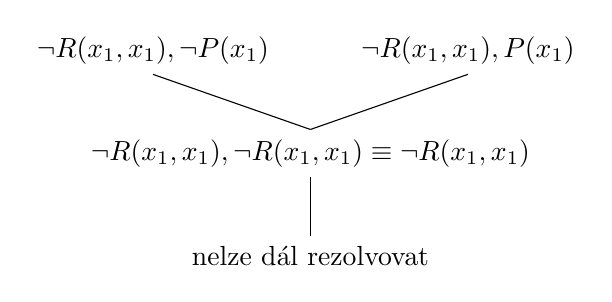
\begin{tikzpicture}[
grow'=up,
note/.style={font=\footnotesize,black!65},
level/.style={sibling distance=4cm},
level distance =1.3cm,
parent anchor=north,
child anchor=south]
\node {nelze dál rezolvovat}
    child {node {$ \neg R(x_1,x_1),\neg R(x_1,x_1) \equiv \neg R(x_1,x_1) $}
        child {node {$ \neg R(x_1,x_1), \neg P(x_1) $}}
        child {node {$ \neg R(x_1,x_1),P(x_1) $}}};
\end{tikzpicture}